\documentclass[10pt,letterpaper]{article}
\usepackage{geometry}
\geometry{margin=1in}
\usepackage{graphicx}
\usepackage[dvipsnames]{xcolor}

\setlength{\parindent}{0pt}
\setlength{\parskip}{0.5em}

%make lists tighter
\usepackage{enumitem}
\setlist{nolistsep}

%reduce spacing before and after section
\usepackage{titlesec}
% reduce section, subsection, etc spacing
\usepackage{titlesec}
\titlespacing*{\section}{0pt}{0\baselineskip}{0\baselineskip}
\titlespacing*{\subsection}{0pt}{0\baselineskip}{0\baselineskip}
\titlespacing*{\subsubsection}{0pt}{0\baselineskip}{0\baselineskip}

%reduce list spacing
\usepackage{enumitem}
\setlist{nosep}

\usepackage[hidelinks]{hyperref}
\usepackage{biblatex}
\usepackage{amsmath}
\usepackage{amsfonts}
\usepackage{amssymb}
\addbibresource{citations.bib}

\usepackage{booktabs}


\title{Lab 3.1 - FMRI, Stat 214, Spring 2025}

% submission must not contain any of your names
% but feel free to make a version for yourself with your names on it
\author{Anonymous}

\begin{document}
\maketitle

\section{Introduction}
Understanding how the human brain processes the rich and complex information embedded in natural language is a central challenge in neuroscience and cognitive science. Encoding models provide a robust computational framework to investigate this, aiming to predict neural activity recorded via functional Magnetic Resonance Imaging (fMRI) directly from features of the language stimuli presented. The fMRI Blood-Oxygen-Level-Dependent (BOLD) signal offers a window into brain function, allowing us to map language processing across different brain regions (voxels). Developing models that accurately predict these BOLD responses can reveal how linguistic information is represented and transformed within the brain.

This lab utilizes an fMRI dataset from \cite{jain2018incorporating}, capturing whole-brain BOLD signals from two subjects as they listened to several hours of natural narrative podcasts. Our goal in Lab 3.1 is to build encoding models that predict these voxel-level brain responses based on the textual content of the podcasts. We will begin by exploring methods to convert the raw text of the stories into embeddings. Specifically, we will implement and compare three distinct embedding techniques: a foundational Bag-of-Words approach, and two widely-used pre-trained embedding methods, Word2Vec \cite{mikolov2013efficient} and GloVe \cite{pennington2014glove}. These embeddings, after appropriate preprocessing steps including downsampling and incorporating temporal delays, will serve as the feature inputs to our predictive models. We will then employ Ridge Regression to model the relationship between these text features and the measured fMRI signals. The performance of models derived from each embedding method will be evaluated using cross-validation and correlation coefficients (CC) to determine which text representation strategy most effectively captures the neural correlates of language comprehension as measured by fMRI.

\section{EDA}
In this section, we will conduct primitive EDA on the dataset, to gain a basic understanding of the data and its structure. The dataset consists of fMRI signals from two subjects, each listening to 101 stories. We divide the data into training/validation and test sets, with 75\% of the stories (75 stories) used for training and validation, and 25\% (26 stories) reserved for testing. The test data is reserved until the Test Performance section, and the EDA and modeling parts are conducted on the training/validation data only. 

In this section, we conducted the EDA on the stories and fMRI signals separately.

\subsection{Stories}
The stories are stored in a "list of words" format, where each story is represented as a list of words, without punctuation or spaces. Figure \ref{fig:story_length} shows the distribution of story lengths, measured by the number of words, across the 75 stories in the training/validation set. The histogram indicates a roughly unimodal distribution with a slight right skew. The majority of stories cluster around the central tendency, with the mean length being 1893 words and the same median length. The similarity between the mean and median confirms the relatively mild skew. The shortest story contains 697 words, while the longest contains 3476 words, showing a considerable range in the duration of the stimuli presented.

\begin{figure}[ht]
    \centering
    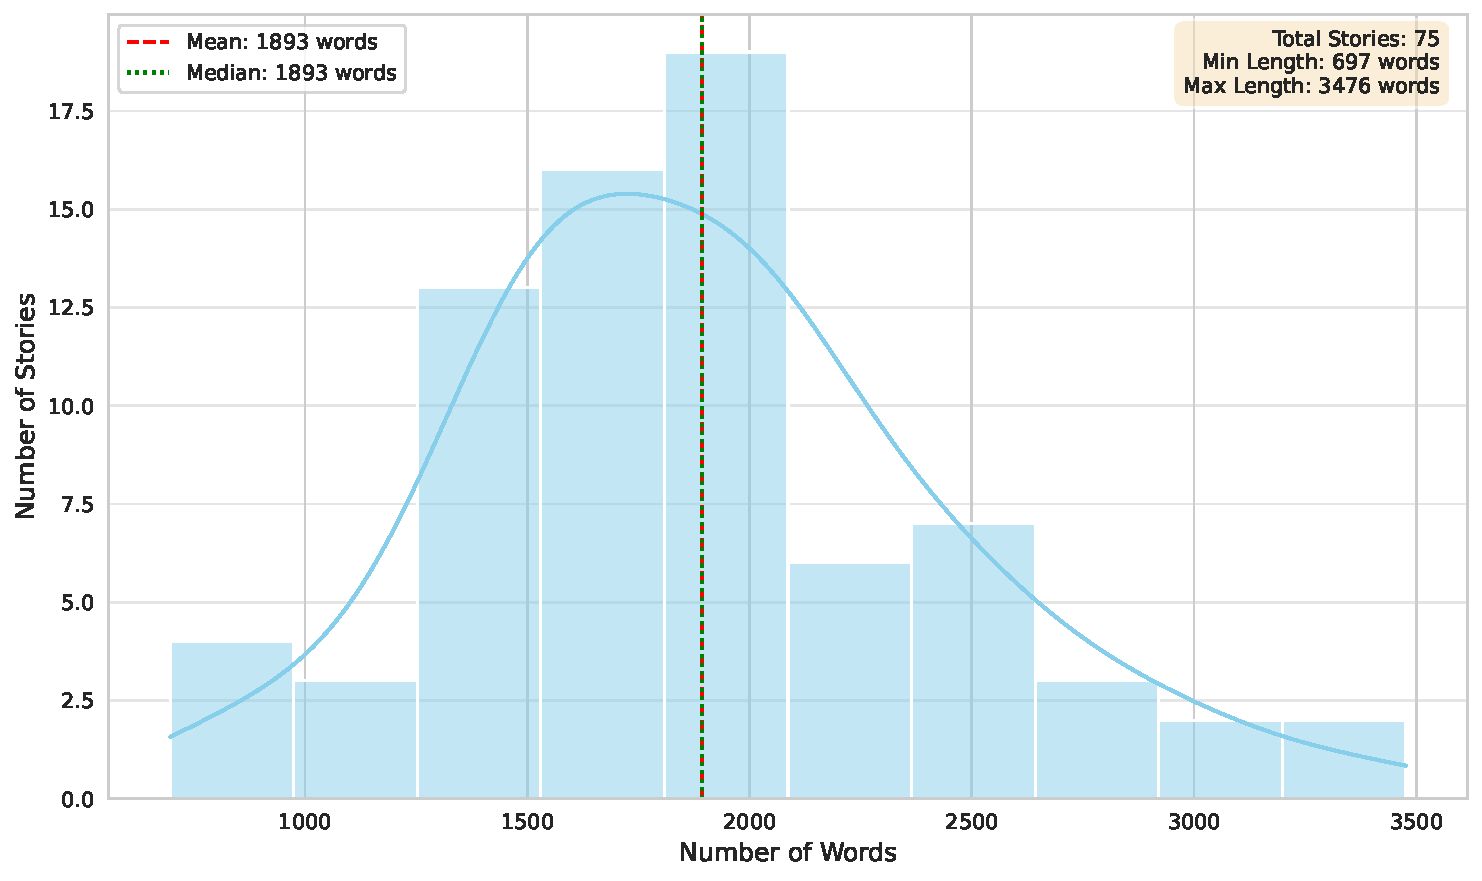
\includegraphics[width=0.8\textwidth]{figs/story_length_distribution.pdf}
    \caption{Distribution of story lengths in training/validation dataset.}
    \label{fig:story_length}
\end{figure}

The following shows a selected piece of one of the stories. The punctuations are added by us as it is not in the original text.

\begin{quotation}
    "My story begins, I am driving my uh silver station Volvo uh from Brooklyn to my mother's house in Rosedale, Queens, on a hot mid-afternoon August day in two thousand and three. My mother uh is a widow. Uh, my father has passed away from lung cancer fifteen years before, nineteen eighty-eight, and she has not resumed dating. She has sworn off men in no uncertain terms. She has told me that, "I am never, ever going to wash another pair of men's underwear again. I am finished with the species. I'm done."
\end{quotation}

The story is a narrative piece, and the text is rich in detail and context. The language is conversational, with a mix of personal anecdotes and reflections. The use of "uh" indicates a speech pattern that is common in spoken language. That implies the corpus is informal and could differ from more formal ones that commonly used in NLP-related tasks.

\subsection{fMRI Signals}
The fMRI signal data captures the brain's response, measured via the Blood-Oxygen-Level-Dependent (BOLD) signal, as subjects listened to the stories. For each of the 75 stories comprising the training/validation set for a given subject, the data is organized into a two-dimensional numerical array. Each row in this array represents the brain activity across all measured voxels at a specific Time of Repetition (TR), which is the sampling interval of the fMRI scanner. Each column corresponds to a single voxel, with 94251 voxels for Subject 2 or 95556 for Subject 3, recorded per subject. Consequently, the dimensions of these arrays are \(T \times V\), where \(V\) is constant, and \(T\) (the number of TRs) varies from story to story, reflecting the differing lengths of the narratives; indeed, as shown in Figure \ref{fig:word_count}, there is a strong positive correlation between the number of words in a story and the duration of its corresponding fMRI recording in TRs.

\begin{figure}[ht]
    \centering
    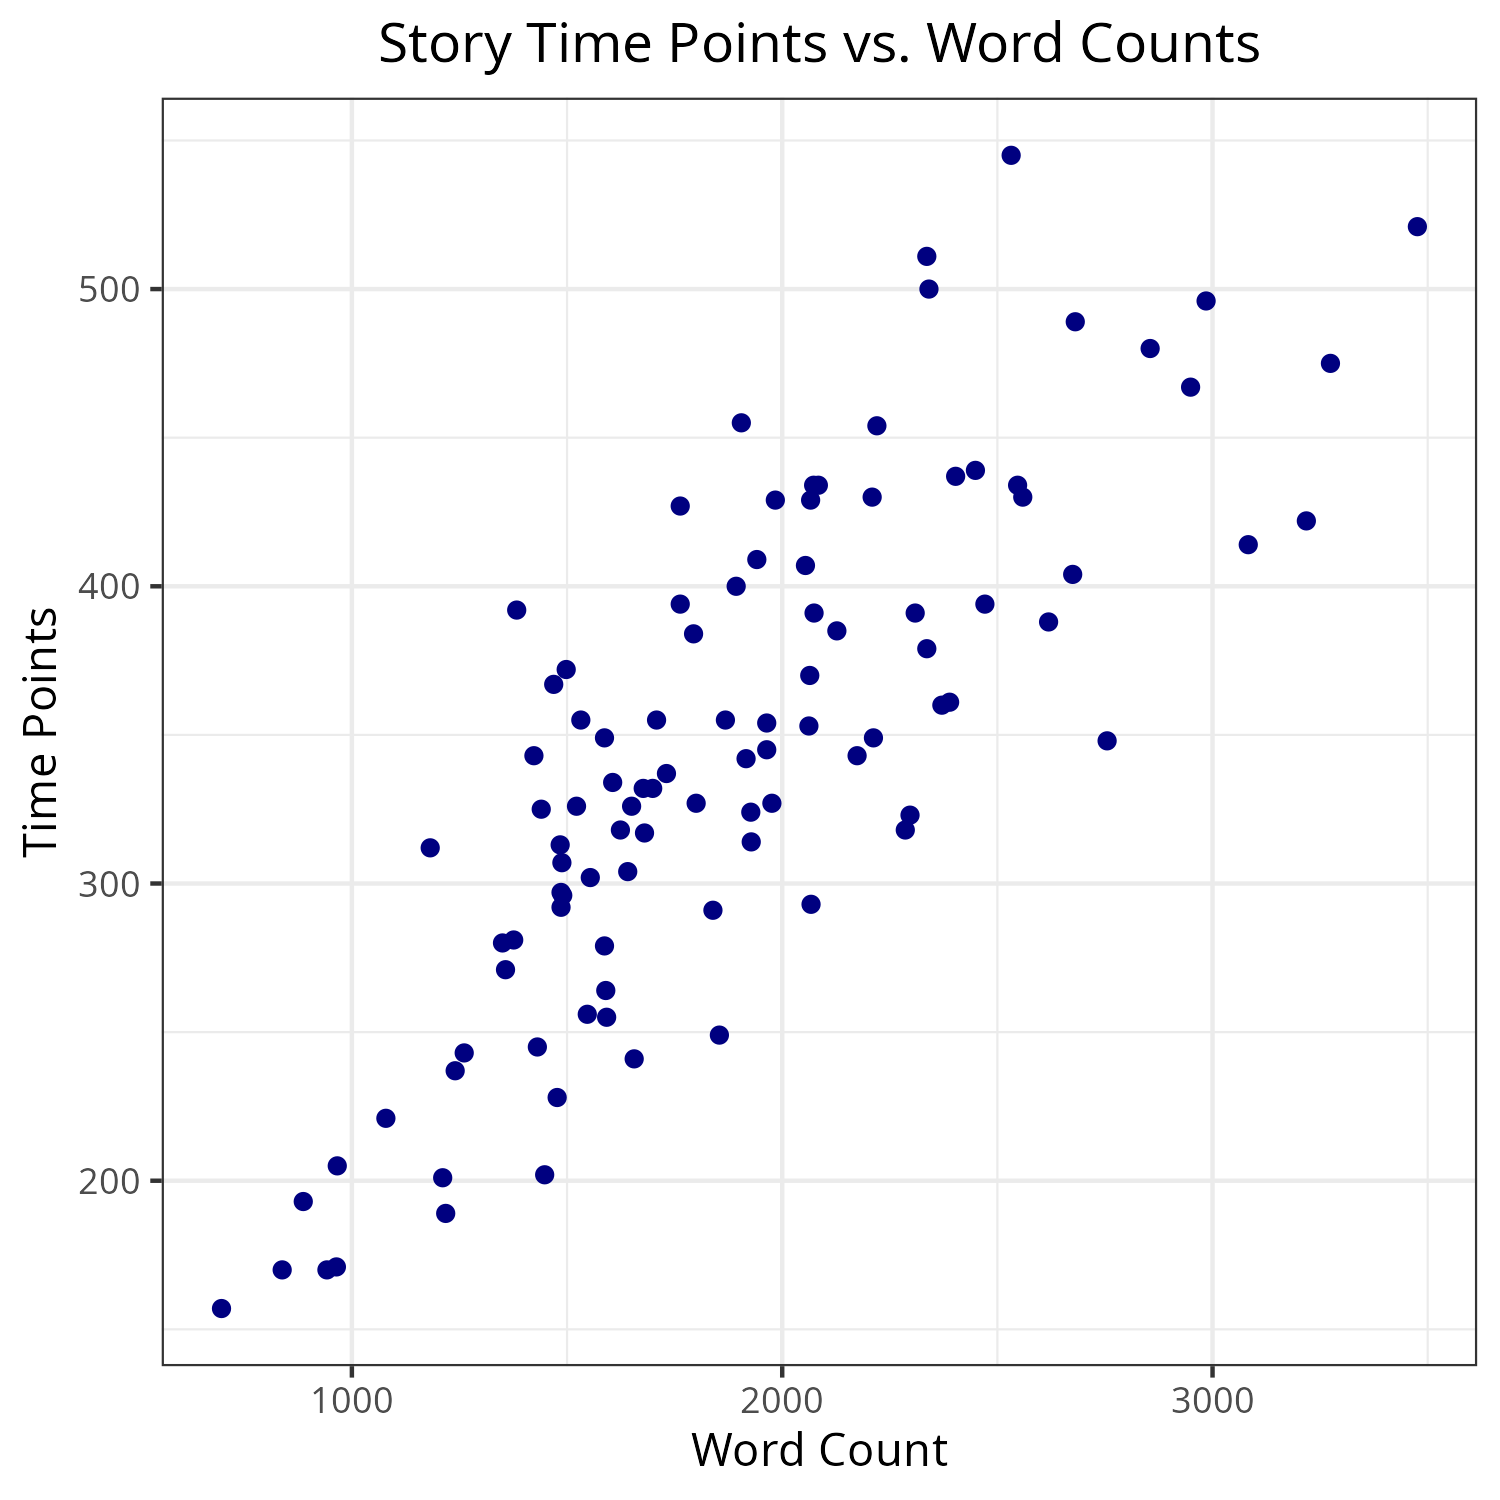
\includegraphics[width=0.6\textwidth]{figs/word_count.png}
    \caption{The number of words in a story is strongly correlated with the number of fMRI repetition time points.}
    \label{fig:word_count}
\end{figure}

To understand the basic characteristics of the BOLD signal itself, we examined the distribution of raw signal values across all voxels and time points within the training/validation set. Since plotting every single reading is impractical, we randomly sampled 10,000 individual signal values from the training data for each subject. Figure \ref{fig:fmri_signal} displays the resulting histograms for these sampled raw BOLD values for Subject 2 and Subject 3. Both distributions appear highly similar, exhibiting an unimodal, approximately Gaussian form centered very close to zero. The spread or variance of the raw signals also seems comparable between the two subjects.

\begin{figure}[ht]
    \centering
    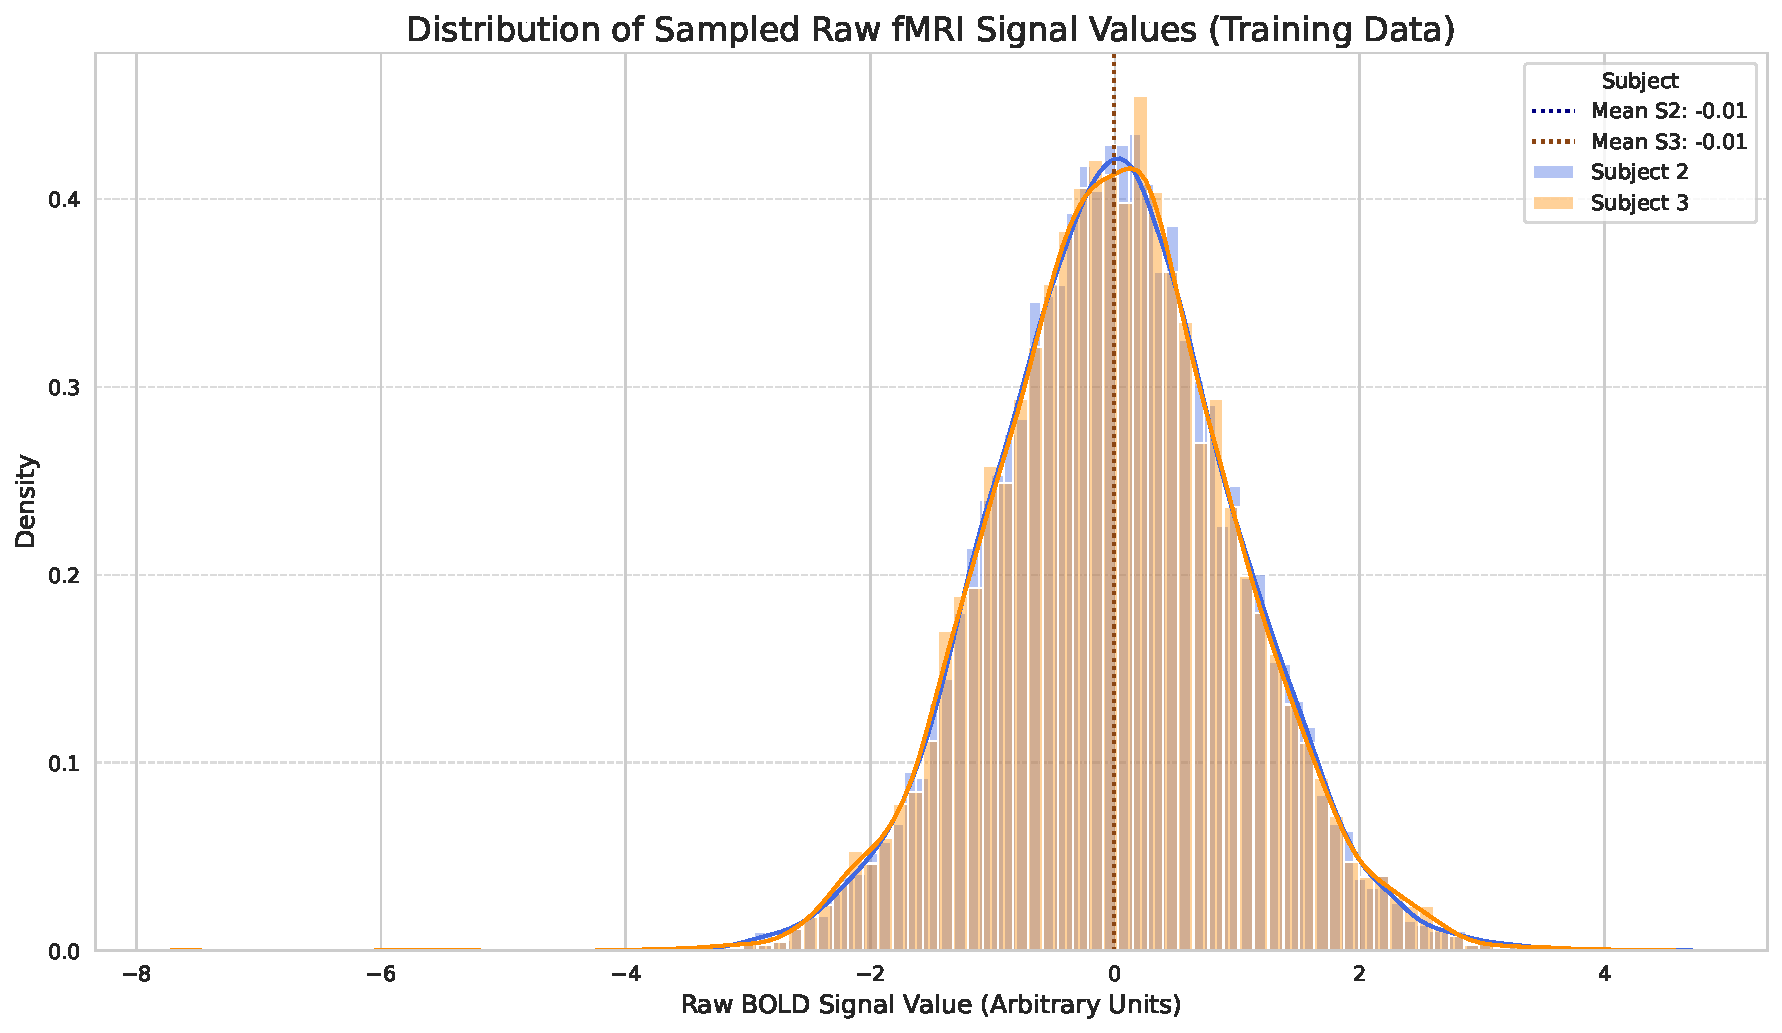
\includegraphics[width=0.8\textwidth]{figs/fmri_signal_distribution.pdf}
    \caption{Distribution of fMRI signals in training/validation dataset.}
    \label{fig:fmri_signal}
\end{figure}

In addition to examining the average fMRI signal across the entire dataset, it is informative to visualize the distribution of signals for each story individually. Figure \ref{fig:boxplots} presents the distribution of several summary statistics (mean, median, interquartile range (IQR), minimum, and maximum) computed from the fMRI signal for each of the 101 stories, where each story is treated as a single data point. The central tendency and spread (IQR) appear highly consistent across stories, while the minimum and maximum values show much greater variability. This variation in extremes may reflect story-specific events or transient noise artifacts.

\begin{figure}[ht]
    \centering
    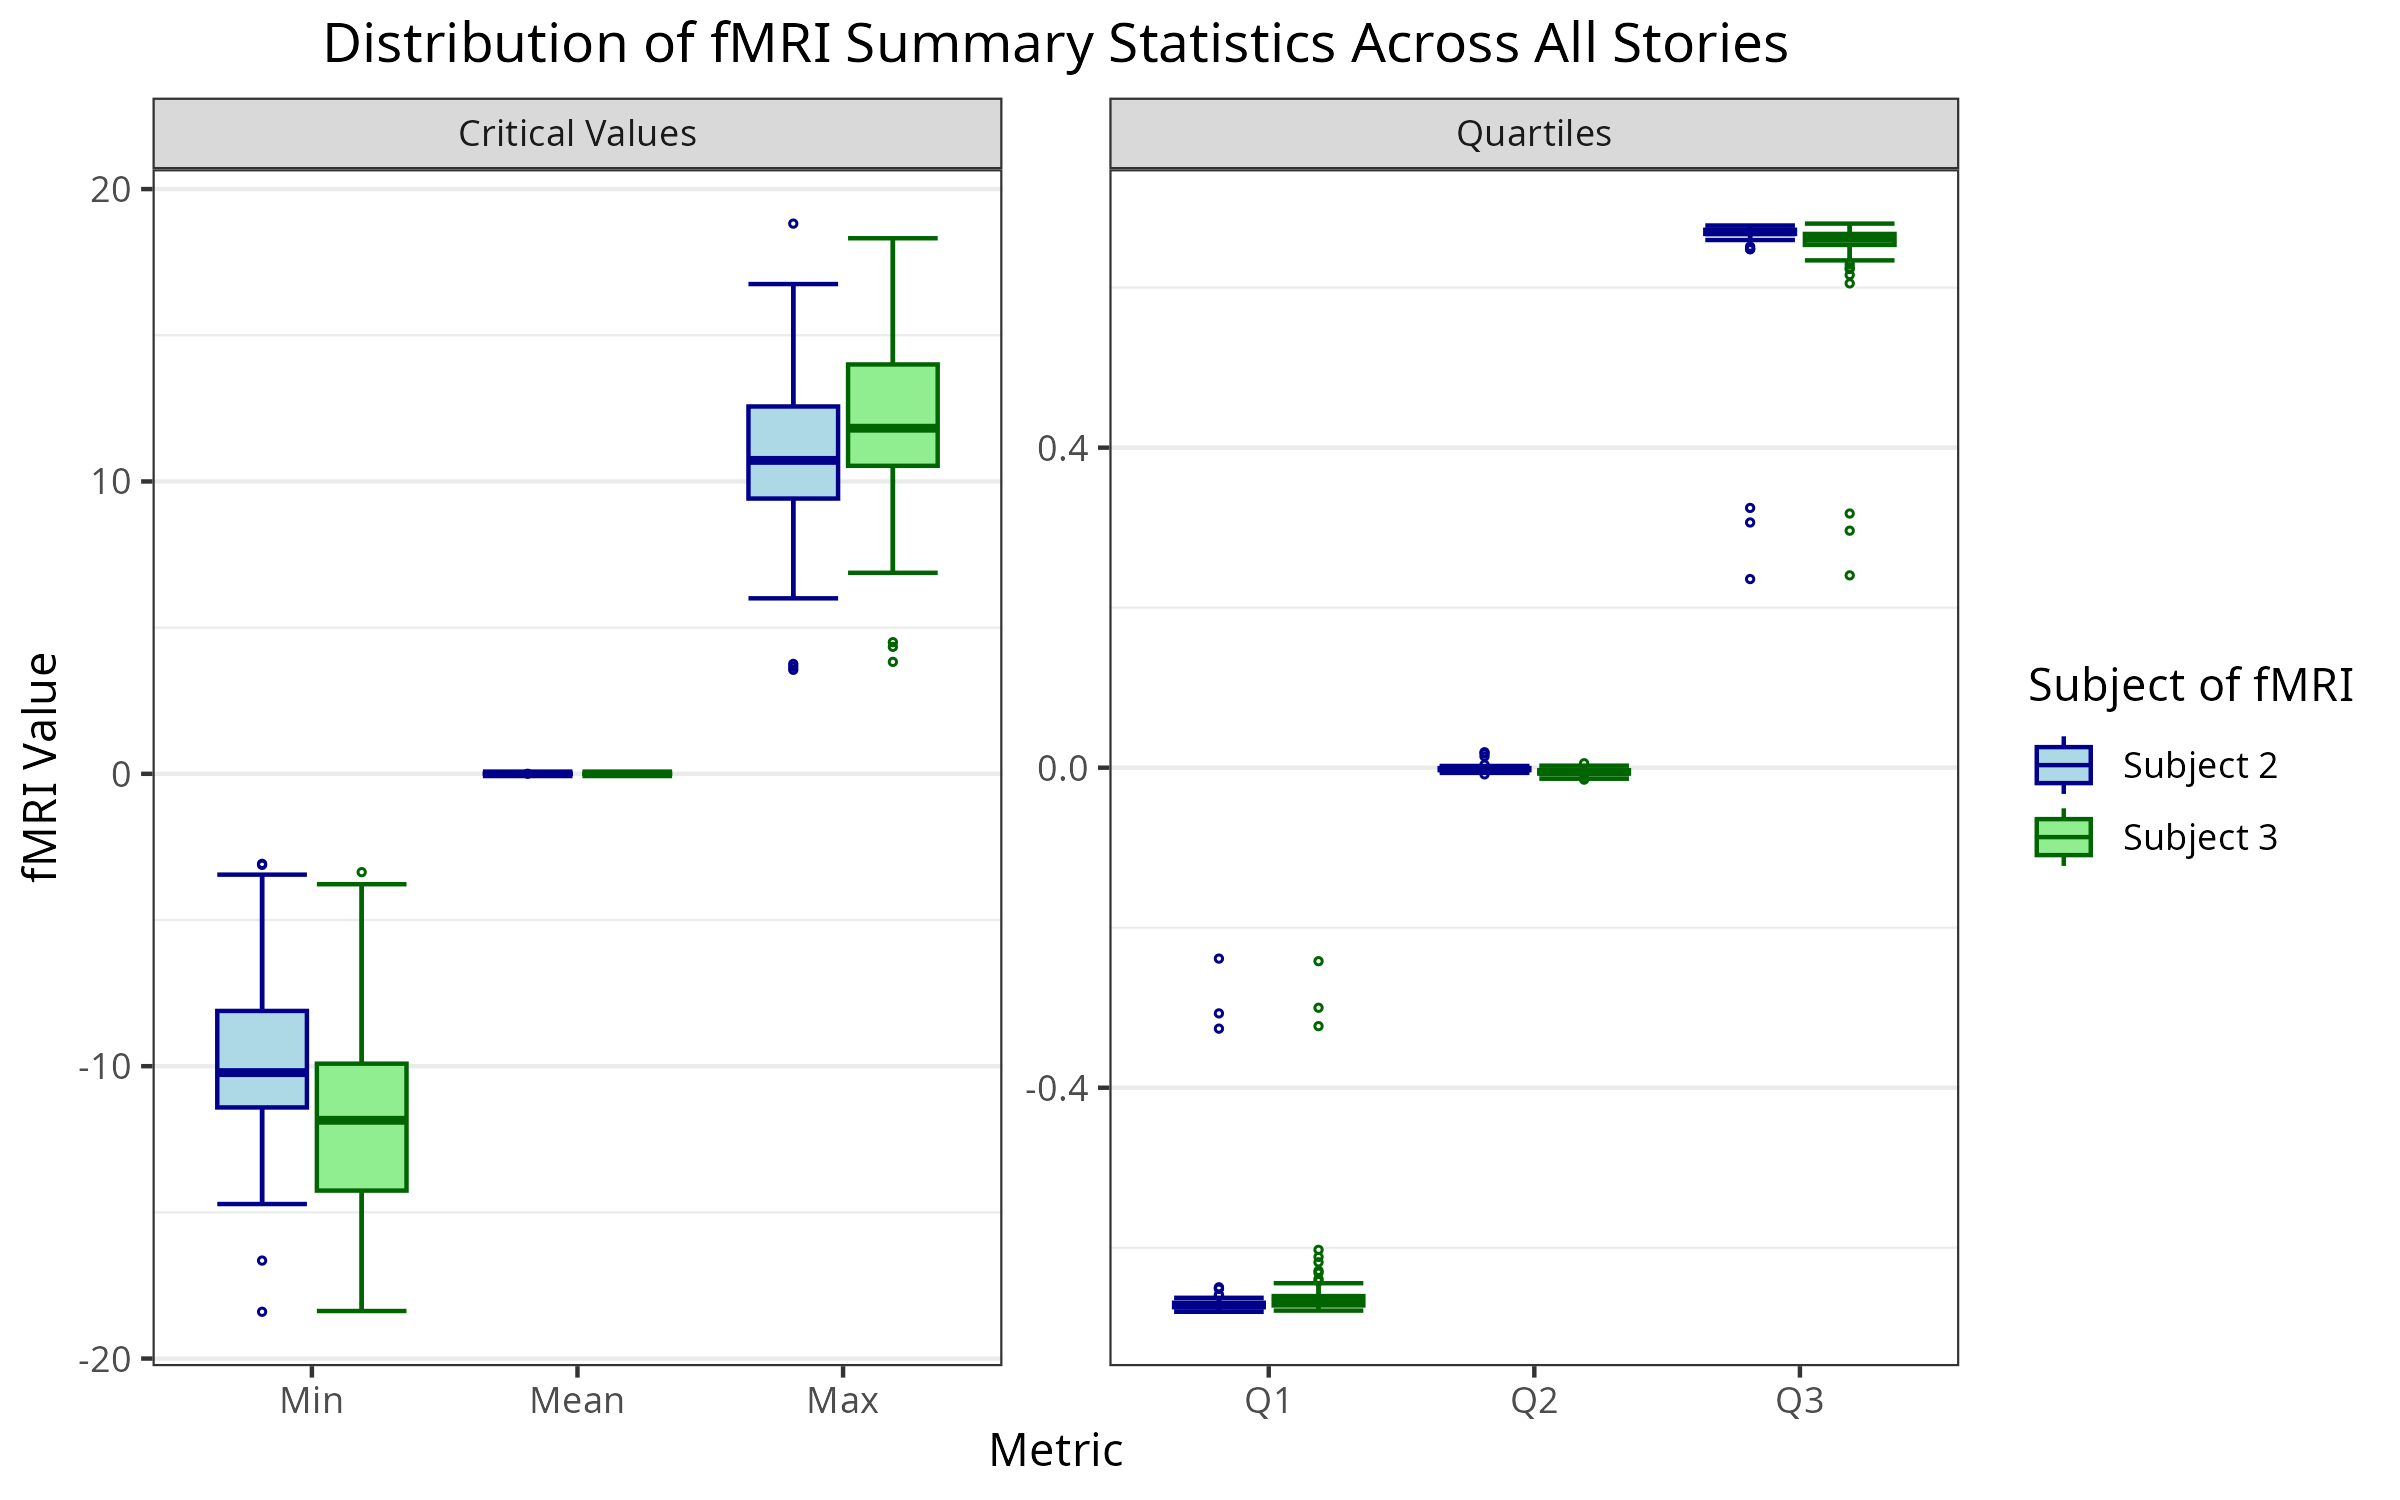
\includegraphics[width=0.8\textwidth]{figs/boxplots.png}
    \caption{Across all 101 stories, the mean, median, and interquartile range (Q1–Q3) of fMRI signals are tightly distributed, while the minima and maxima show wide variation.}
    \label{fig:boxplots}
\end{figure}

Figure \ref{fig:mean_signal} offers a more granular view by plotting the mean and IQR of the fMRI signal across all voxels at each time point within selected example stories. This enables a direct comparison of the temporal signal profiles between Subject 2 and Subject 3 over the course of each story. Despite some fluctuations, the mean signal values for both subjects consistently oscillate within a relatively narrow range (approximately –1 to 1), not only in the stories shown here but across the full set.

\begin{figure}[ht]
    \centering
    \parbox{\textwidth}{\centering 
        \fontsize{13pt}{13pt}\selectfont \textbf{Average fMRI Signal Across Selected Stories}  
        {\fontsize{11pt}{13pt}\selectfont Mean (line) and IQR (shaded) comparison between   \textcolor{RoyalBlue}{\textbf{Subject 2}} and \textcolor{ForestGreen}{\textbf{Subject 3}}.} 
    }
    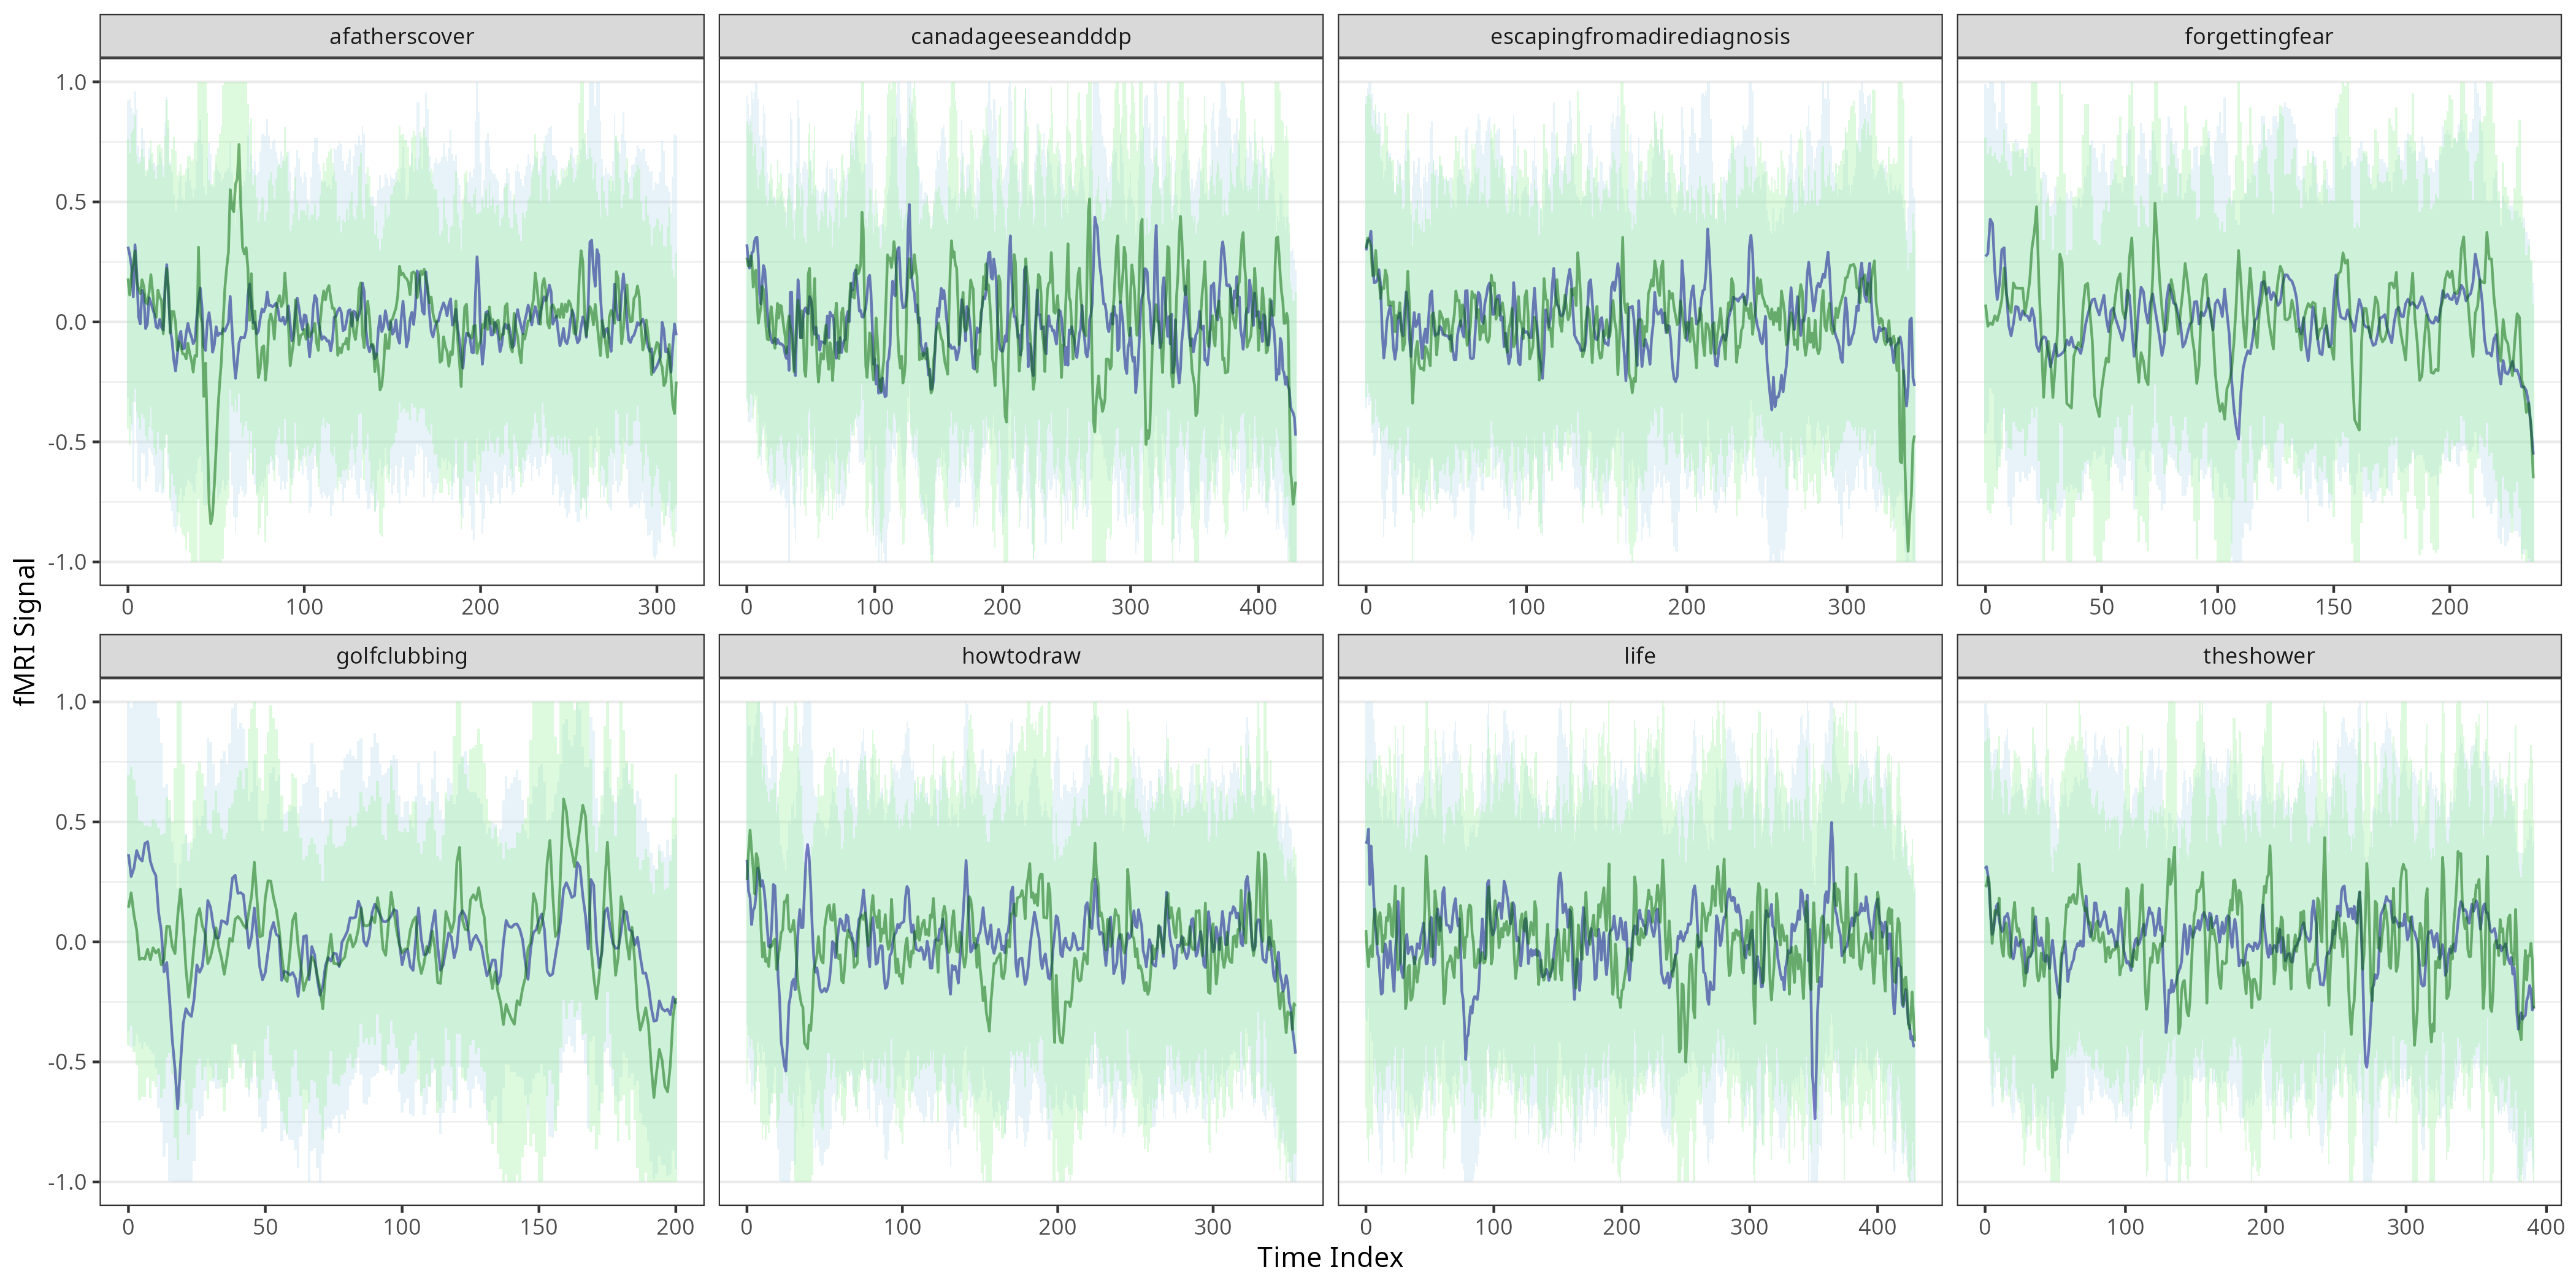
\includegraphics[width=\textwidth]{figs/mean_signal.png}
    \caption{Mean fMRI signal (line) and interquartile range (shaded area) for Subject 2 and Subject 3 at each time point, plotted separately for each story. Mean values for both subjects generally oscillate between –1 and 1.}
    \label{fig:mean_signal}
\end{figure}

In stark contrast, the maximum signal value at each time point, shown in Figure~\ref{fig:max_signal}, reveals substantial variability in peak activity levels over the course of a single story. Although some of this variation may be driven by noise, there appears to be a moderate degree of correlation or shared structure in the timing of peak signal fluctuations between the two subjects listening to the same story.

\begin{figure}[ht]
    \centering
    \parbox{\textwidth}{\centering 
        \fontsize{13pt}{13pt}\selectfont \textbf{Maximum fMRI Signal Across Selected Stories}  

        {\fontsize{11pt}{13pt}\selectfont Comparison between \textcolor{RoyalBlue}{\textbf{Subject 2}} and \textcolor{ForestGreen}{\textbf{Subject 3}}.} 
    }
    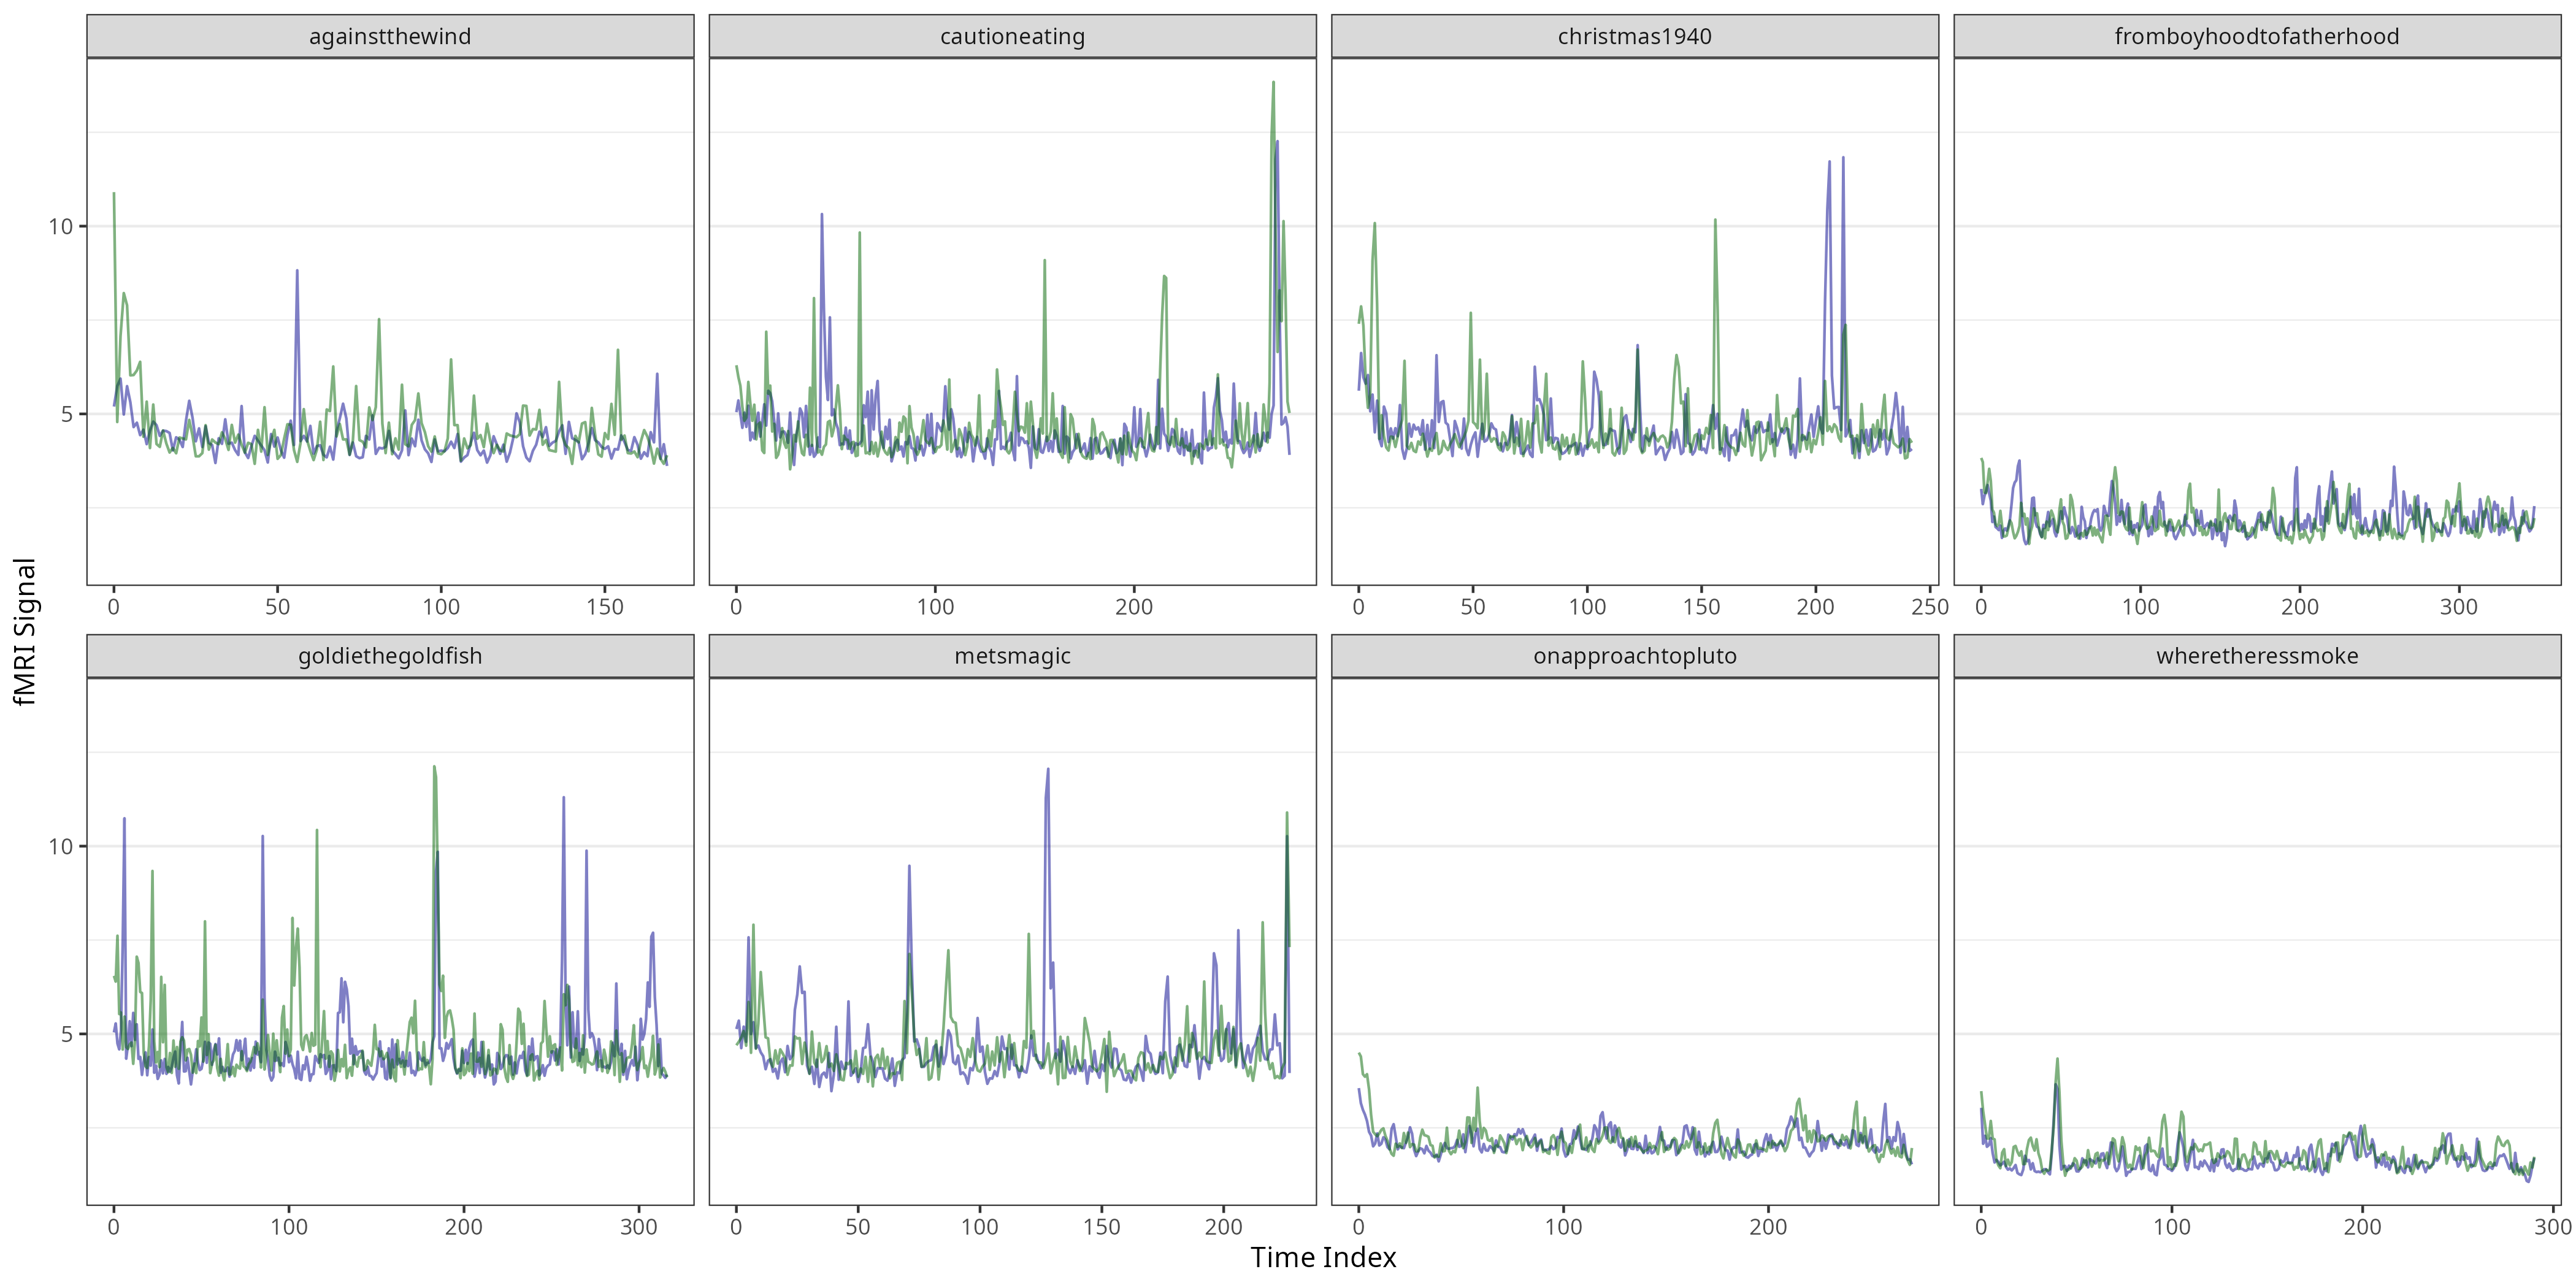
\includegraphics[width=\textwidth]{figs/max_signal.png}
    \caption{Maximum fMRI signals for Subject 2 and Subject 3 are highly moderate across several stories, despite substantial noise.}
    \label{fig:max_signal}
\end{figure}

Another thing to note is that the fMRI signals of Subject 2 contain some NaN values, which are not present in Subject 3. However, the proportion of NaN values is very small, only \(5.9 \times 10^{-6}\) of the total number of values. Due to the small proportion, we simply imputed them with global mean to prepare the prediction and expect no significant impact on the model performance no matter which imputation method we use.

\section{Embeddings}
To predict brain activity (fMRI signals) from the podcast stimuli the subjects listened to, we first need to convert the raw text of the stories into a numerical format that can be used as input features for a predictive model. This process involves creating vector representations for the text data, which is embedding. As the lab instructions suggest, we will use a three-stage approach to generate these embeddings. The first stage involves creating word-level embeddings, with bag-of-words and pre-trained embeddings (Word2Vec and GloVe). Then in the second stage, we aggregate these word-level embeddings into chunk-level representations that correspond to the fMRI time series one-by-one. The third stage is a temporal-aware feature engineering that incorporates the past embeddings into the current chunk-level representation, to allow the model to capture the impact of the previous story chunks on the current fMRI signal. We explain each of these stages in detail below.

\subsection{Word-level embeddings}
As the code provided in the lab instructions suggests, we tokenize the text data into words divided by spaces and punctuations, instead of Byte Pair Encoding or other tokenization methods used in modern NLP models. Then various techniques can be used to create an embedding for each word. The most common methods are Bag of Words (BoW) and pre-trained embeddings such as Word2Vec and GloVe.

\subsubsection{Bag of Words (One-hot encoding)}
The Bag-of-Words (BoW) model is a basic technique in NLP processing for representing text data numerically. It simplifies text by treating it as an unordered collection (or "bag") of words, disregarding grammar and word order, but keeping track of word frequency.

When applied strictly at the individual word level, as in the initial stage of our embedding process, the BoW representation becomes a one-hot encoding. Each unique word in the vocabulary is assigned a unique index, and its embedding is a sparse vector with a 1 at that index and 0s elsewhere. This differs from the standard application of BoW, which typically involves aggregating word counts or embeddings across a larger text unit like a document or, in our case, a time chunk corresponding to an fMRI TR. As the subsequent Lanczos resampling step aggregates these word-level one-hot vectors into chunk-level representations, the result preserves some temporal dynamics within the chunk. This contrasts with a standard chunk-level BoW (e.g., summing the one-hot vectors within a chunk), which would assign a single, static embedding to the entire chunk.

Despite the aggregation method, this approach retains the core characteristic of BoW: it does not capture semantic meaning or relationships between words. Each word is treated as a distinct, independent feature, and the model considers all pairs of different words to be equally dissimilar.

Notably, for all words that appear in the training set only once, we assign a unique to represent all of them. This is done because the model can not learn meaningful information from a word that appears only once. Also, it enables the model to learn how to deal with out-of-vocabulary words, as we put new words in the validation and test sets into this unique index. It reduces the dimensionality of the embedding, too.

The final dimension of the BoW embedding is [approx 5000, pending], far larger than the other two methods, and the embedding is largely sparse.

\subsubsection{Pre-trained embeddings: Word2Vec and GloVe}
In contrast to Bag-of-Words, methods like Word2Vec \cite{mikolov2013efficient} and GloVe \cite{pennington2014glove} generate dense, low-dimensional (300 dimensions) embeddings that capture semantic relationships between words. Instead of treating words as isolated units, these techniques learn vector representations where words with similar meanings or that appear in similar linguistic contexts are positioned closer together in the vector space.

The fundamental idea behind Word2Vec is that a word's meaning can be inferred from its surrounding words. It learns embeddings by training a neural network to predict either context words given a central target word (Skip-gram model) or the target word given its context (Continuous Bag-of-Words model).

GloVe (Global Vectors for Word Representation) takes a different approach, focusing on global corpus statistics. It learns word vectors such that their dot product equals the logarithm of their co-occurrence probability, capturing meaning implicitly encoded in word co-occurrence patterns across a vast amount of text.

For this project, we utilize pre-trained versions of Word2Vec and GloVe models. These models have been trained on massive corpora, allowing them to learn general-purpose semantic representations. Using pre-trained embeddings offers an advantage as they bring in semantic information and potentially lead to better predictive performance for the fMRI signals compared to the semantically agnostic BoW approach because they capture the similarities and relationships between words. This is particularly important in our case, where the human brain understands language semantically.

These pre-trained models provide dense vector representations for each word in their vocabulary, which we then use as the initial word-level features before aggregation and temporal processing.

\subsection{Chunk-level Aggregation with Lanczos Resampling}

The word-level embeddings generated in the previous step provide a representation for each word occurring at specific time points in the story. However, the fMRI signals we aim to predict are measured at discrete time intervals, known as Repetition Times (TRs). During a single TR, multiple words may be presented to the subject. Therefore, the sequence of word embeddings (with dimensions \(\text{num\_words} \times \text{embedding\_dim}\)) needs to be aggregated to match the temporal resolution of the fMRI data, resulting in a single embedding vector for each TR (dimensions \(\text{num\_TRs} \times \text{embedding\_dim}\)).

To achieve this temporal alignment and aggregation, we employ Lanczos interpolation given in the instruction, a commonly used technique for signal resampling. This method calculates the embedding representation for each TR time point by applying a weighted average (convolution) to the surrounding word-level embeddings. The weights are determined by the Lanczos kernel, which is a windowed sinc function. Specifically, the weight assigned to a word embedding at time \(t_{word}\) when calculating the aggregated embedding for TR center time 
\(t_{TR}\) is given by the Lanczos kernel function \(L(t)\):

\[
L(t) = \text{sinc}(\pi t f_c) \cdot \text{sinc}(\frac{\pi t f_c}{a}) \cdot \mathbb{I}(|t f_c| < a)
\]

where \(t = t_{TR} - t_{word}\) is the time difference, $f_c$ is the cutoff frequency, $a$ is the window size parameter, and \(\text{sinc}(x) = \frac{\sin(x)}{x}\).

In signal processing, the Lanczos kernel minimizes aliasing artifacts that can arise when downsampling and provides a good balance between smoothing noise and preserving the relevant temporal structure, compared to simpler methods like rectangular window averaging or nearest-neighbor interpolation. Applying the Lanczos kernel on word sequence is heuristic because the word embeddings are not continuous, and dramatically changing in a short time is reasonable and expected. However, it still provides an effective way to aggregate the word-level embeddings into chunk-level representations that align with the fMRI TRs.

\subsection{Temporal Feature Engineering}

The brain contextually processes language, and the semantic meaning interpreted at any moment is influenced by preceding words and sentences. Therefore, the brain activity measured in a specific TR is likely influenced not only by the stimuli presented during that TR but also by the stimuli from the recent past.

To account for these temporal dependencies, we engineer features that incorporate information from previous time points. Following the aggregation step, each TR has an associated embedding vector. We augment this representation by concatenating the embedding vectors from preceding TRs. Specifically, for each TR at time \(t\), we take aggregated embedding vectors from times \(t-1\), \(t-2\), \(t-3\) and \(t-4\) TRs and concatenate them. Notice that the embedding vector for the current TR, \(t\) is not included in the augmented representation, for consistency with the instruction.

This creates a temporally expanded feature vector for each TR. If the original aggregated embedding dimension was \(d\), the resulting feature dimension becomes \(4d\). This allows the subsequent predictive model to potentially capture the influence of stimuli presented prior to the brain activity measured at the current TR.

\section{Modeling}

\subsection{Modeling Approach}
We create a predictive model to predict fMRI levels for each voxel using the embeddings we have generated. Specifically, we fit a ridge regression model. This modeling approach contains the parameter alpha, which controls the penalty term on the model's weights as L2 (squared) loss.

We start by fitting a regression model for Subject 2, for each different embedding - Bag of Words, GloVe, and Word2Vec. Using the cross-validation strategy described in the next section, we find the best alpha hyperparameter value for regularization.

\subsection{Model Evaluation Strategy}

We utilize a standard k-fold cross-validation strategy to develop our predictive models. The split is done at a story level instead of a TR level to mimic the real-world scenario where the model is trained on a set of stories and then evaluated on unseen stories. 60\% of the stories are used for training and validation, and the remaining are reserved for testing and remain untouched until the final evaluation.

For each fold, the bag-of-words is retrained on the training data to avoid data leakage, while the pre-trained embeddings are applied before the data split as they are fixed and independent of the training data.

The metric we use to evaluate the model performance is the correlation coefficient (CC) between the predicted and actual fMRI signals, which is a standard metric in the context of fMRI signals. We do this per voxel, giving us a voxel-wise CC. This is the metric that our model is trained to optimize for.

This strategy is designed to mimic the real-world scenario with the best efforts to avoid data leakage and measure the model's generalization performance.

\subsection{Results}

Our cross-validation results for hyperparameter tuning are shown in Tables \ref{tab:word2vec_cv}, \ref{tab:glove_cv}, and \ref{tab:bow_cv} for the models trained with the Word2Vec, GloVe, and Bag of Words embeddings, respectively. These are performance metrics on the validation set.


\begin{table}[ht]
\centering
\caption{Performance metrics for Word2Vec at different values of \texttt{alpha}. 
Best alpha: 1000 (Mean CV CC = 0.0067).}
\label{tab:word2vec_cv}
\begin{tabular}{cccccc}
\toprule
\textbf{Alpha} & \textbf{Mean CC} & \textbf{Median CC} & \textbf{Top1 CC} & \textbf{Top5 CC} & \textbf{Top10 CC} \\
\midrule
0.1   & 0.0035 & 0.0032 & 0.0462 & 0.0462 & 0.0325 \\
1     & 0.0037 & 0.0034 & 0.0460 & 0.0462 & 0.0332 \\
10    & 0.0036 & 0.0031 & 0.0468 & 0.0421 & 0.0340 \\
100   & 0.0039 & 0.0032 & 0.0442 & 0.0444 & 0.0312 \\
1000  & 0.0041 & 0.0036 & 0.0452 & 0.0429 & 0.0337 \\
\bottomrule
\end{tabular}
\end{table}

\begin{table}[ht]
\centering
\caption{Performance metrics for GloVe at different values of \texttt{alpha}. 
Best alpha: 1000 (Mean CV CC = 0.0061).}
\label{tab:glove_cv}
\begin{tabular}{cccccc}
\toprule
\textbf{Alpha} & \textbf{Mean CC} & \textbf{Median CC} & \textbf{Top1 CC} & \textbf{Top5 CC} & \textbf{Top10 CC} \\
\midrule
0.1   & 0.0036 & 0.0041 & 0.0442 & 0.0462 & 0.0337 \\
1     & 0.0035 & 0.0044 & 0.0450 & 0.0452 & 0.0336 \\
10    & 0.0037 & 0.0041 & 0.0448 & 0.0455 & 0.0340 \\
100   & 0.0039 & 0.0038 & 0.0466 & 0.0451 & 0.0332 \\
1000  & 0.0042 & 0.0039 & 0.0469 & 0.0458 & 0.0333 \\
\bottomrule
\end{tabular}
\end{table}


\begin{table}[ht]
\centering
\caption{Performance metrics for BoW at different values of \texttt{alpha}. 
Best alpha: 1000 (Mean CV CC = 0.0230).}
\label{tab:bow_cv}
\begin{tabular}{cccccc}
\toprule
\textbf{Alpha} & \textbf{Mean CC} & \textbf{Median CC} & \textbf{Top1 CC} & \textbf{Top5 CC} & \textbf{Top10 CC} \\
\midrule
0.1   & 0.0019 & 0.0020 & 0.0423 & 0.0432 & 0.0312 \\
1     & 0.0021 & 0.0018 & 0.0435 & 0.0442 & 0.0325 \\
10    & 0.0023 & 0.0022 & 0.0440 & 0.0448 & 0.0331 \\
100   & 0.0028 & 0.0025 & 0.0442 & 0.0430 & 0.0345 \\
1000  & 0.0031 & 0.0029 & 0.0451 & 0.0435 & 0.0337 \\
\bottomrule
\end{tabular}
\end{table}

From this cross-validation process, the best model ended up being the Bag of Words model which used an alpha of 1000. It had a mean test CC of 0.0009, median CC of 0.0009, Top 1 percentile CC of 0.0311, and Top 5 Percentile CC of 0.0215. Overall, the CC is low (our model has a limited ability to predict fMRI levels well), and slightly higher than a random guessing.


\subsection{Detailed Evaluation \& Analysis}
For the model with the best embedding, which was Bag of Words, we performed a more detailed evaluation. We examine the distribution of test CC across voxels. We generate a list of CCs (one for each voxel), then visualize see how the CC is distributed across voxels. We are looking to see how differently the model performs on some voxels in comparison with others if they all have similar performance, or if there is a skew/outlier voxels, etc. Figure \ref{fig:cc_dist_voxels_subject_2} describes the distribution of CC across voxels. We can see that the distribution is relatively symmetric, with no major skew. Numerically, the distribution of CC is centered around 0.0009, with a 25th percentile above -0.01 and a 75th percentile at approximately 0.01. An important note is that there are numerous outlier voxels on either side (based on the 1.5*IQR outlier threshold), which suggests that the spread of CC across voxels is relatively large. The positive outliers are stronger/slightly further from the center than the negative outliers.

So, this model does not perform the same across all voxels. Scientifically, this implies that prediction in different voxels of the brain has varying levels of difficulty. This could stem from that some brain areas (voxels) are irreverent from language processing, or at least language processing in listening to these stories, leading to noise that cannot be predicted with the story text, while some others actively respond to the story. However, more domain knowledge is required to justify the hypothesis.

We want to have a reasonable interpretation criterion for interpreting voxels according to PCS. We want to make sure that the predictions are meaningfully better than by chance. One option is to only select voxels in the top \(x\) percentile of the observed distribution of CCs (i.e. for \(x=5\) for the 5th percentile). The reason to select the top voxels is that we know they respond to the stories actively, while others could be just random noise, as stated before. In terms of stability, we would ideally want to be able to predict voxels well across different stories, subjects, etc. We could check this by examining each voxel's CC across model performance for different stories, or different models for different subjects. Lastly, we want the full prediction process to be reproducible and computed reliably. These conditions align with the three main parts of PCS.


\begin{figure}
    \centering
    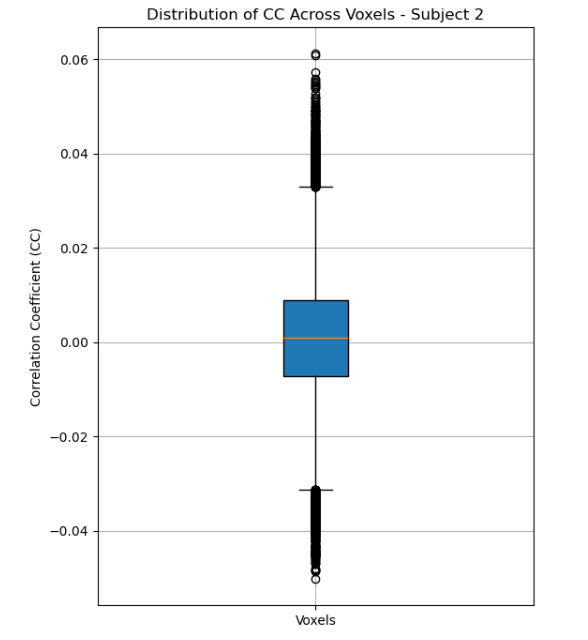
\includegraphics[width=0.5\linewidth]{figs/cc_dist_voxels_subject_2.png}
    \caption{Distribution of CC across voxels for Subject 2.}
    \label{fig:cc_dist_voxels_subject_2}
\end{figure}


\subsection{Stability Analysis}
We conduct a stability analysis by examining performance across different subjects. In this case, we compare Subject 2, which has been detailed so far, with another model trained on Subject 3. We train and test a model on Subject 3 using the same stories as Subject 2. We can then compare the distributions of CCs to see how stable the process is across different subjects.

\begin{table}[ht]
  \centering
  \caption{Test Performance Metrics for Subject 2 and Subject 3}
  \label{tab:subject_performance}
  \begin{tabular}{lcccc}
    \hline
    \textbf{Subject} & \textbf{Mean Test CC} & \textbf{Median Test CC} & \textbf{Top 1 Percentile CC} & \textbf{Top 5 Percentile CC} \\
    \hline
    Subject 2        & 0.0009                & 0.0009                 & 0.0311                     & 0.0215                      \\
    Subject 3        & 0.0017                & 0.0014                 & 0.0320                     & 0.0213                      \\
    \hline
  \end{tabular}
\end{table}




Our final Subject 3 model uses the Bag of Words embedding and an alpha hyperparameter of 1000 for Ridge. After the training, the final test set performance for Subject 3 was a mean CC of 0.0017, median CC of 0.0014, top 1 percentile CC of 0.0320, and a top 5 percentile CC of 0.0213. This is shown in Table \ref{tab:subject_performance}. In comparison with Subject 2, we note that the top 1 percentile and top 5 percentile CCs are very similar, which suggests stable results. The mean and median CC are better for Subject 3, though not by a large margin that would suggest high instability.

We also visualize the distribution of CC across voxels to have a deeper understanding and comparison, with Subject 2. This is shown in Figure \ref{fig:cc_dist_voxels_subject_3}. Visually, the distributions of CC across voxels look very similar between Subject 2 and Subject 3. The medians and quartiles, and outliers also show no major differences. This suggests a generally stable result.

\begin{figure}
    \centering
    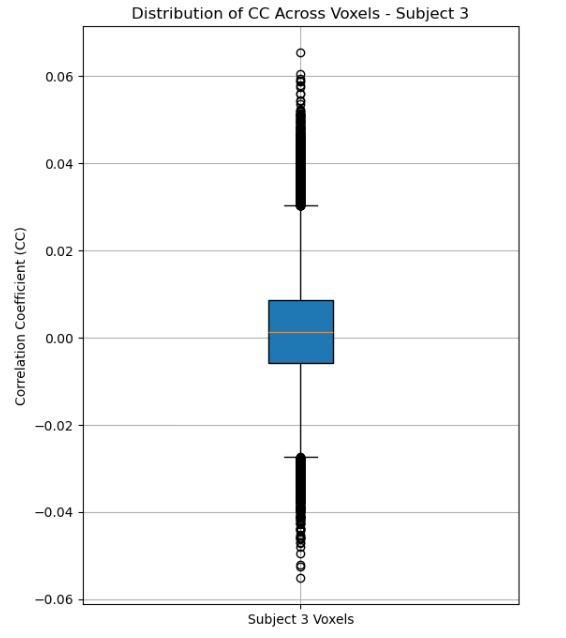
\includegraphics[width=0.5\linewidth]{figs/cc_dist_voxels_subject_3.png}
    \caption{Distribution of CC across voxels for Subject 3.}
    \label{fig:cc_dist_voxels_subject_3}
\end{figure}



\section{Conclusion}
In this lab, we explored the feasibility of predicting fMRI BOLD signals associated with listening to narrative stories using features derived from the story text. We implemented a pipeline that involved generating word-level embeddings using three distinct methods: Bag-of-Words, pre-trained Word2Vec, and pre-trained GloVe. These word embeddings were then aggregated to match the fMRI TRs via Lanczos resampling, and temporally lagged features were incorporated to account for the delay and contextual processing. Finally, Ridge Regression models were trained for each embedding type to predict voxel-level activity, with performance evaluated using cross-validation and correlation CC.

Our results indicated that predicting fMRI signals with this approach is challenging, yielding generally low CC values across all models, suggesting limited predictive power. Surprisingly, the semantically simple BoW model outperformed the models based on pre-trained Word2Vec and GloVe embeddings, achieving the highest average CC during cross-validation, albeit still at a low absolute level. Further analysis of the best-performing BoW model revealed variability in prediction accuracy across different brain voxels, though the overall performance patterns showed reasonable stability when compared across the two subjects.

The weak performance, particularly of the semantically meaningful Word2Vec and GloVe embeddings, points towards a fundamental limitation in relying solely on aggregated word embeddings within a linear modeling framework. Language resampling is additive; the meaning of a sentence is far more complex than a simple linear combination of its constituent word meanings. Operations like negation (e.g., the word "not" altering meaning) or the context-dependent meaning of words are not well captured by linearly averaging pre-computed word vectors using Lanczos resampling.

The better performance of BoW in this specific pipeline might stem from several factors. Firstly, its high dimensionality might preserve more distinct information than low-dimensional dense vectors of Word2Vec/GloVe. Secondly, because BoW embeddings don't encode complex inter-word semantics initially, the linear averaging process might be less detrimental to the simpler information (word presence/frequency) they convey. In essence, the combination of linear aggregation (Lanczos) and a linear predictive model (Ridge) appears ill-suited to leverage the strengths of dense semantic embeddings. This suggests that more sophisticated methods capable of handling non-linear aggregation and context are likely necessary to effectively model the brain's processing of natural language.

\newpage

\printbibliography

\appendix
\section{Academic honesty}
\subsection{Statement}
We affirm that the work in this report is entirely my own. We have not copied from any unauthorized sources, and all contributions from classmates, external sources, or tools are acknowledged. Academic research honesty is necessary because it ensures fairness, builds trust in scholarly work, and reflects personal integrity. Misrepresenting work undermines academic standards and disrespects the time and effort of peers and educators. Maintaining honesty in research fosters a learning environment where collaboration and progress can thrive authentically.

\subsection{LLM Usage}

We used ChatGPT to assist in clarifying concepts, creating visualizations, checking grammar, and improving the structure of our explanations. No content of the report or code was generated by the LLM without our review, editing, and refinement. We ensured that all content was written and understood by us, and the LLM was used as a tool to enhance our work rather than replace our understanding, we take full responsibility for all content in the report.

\end{document}